\addtocounter{exercice}{1}
\paragraph*{Exercices \theexercice~à\addtocounter{exercice}{4}~\theexercice}~\\
\addtocounter{exercice}{-5}

\noindent Le carré $ABCD$ a un côté de longueur 8 cm.\\
$M$ est un point du segment $[AB]$.\\
On dessine dans le carré $ABCD$ :
\begin{itemize}
	\item Un carré de côté $[AM]$
	\item Un triangle isocèle de base $[MB]$ et dont la hauteur a même mesure que le côté $[AM]$ du carré.
\end{itemize}
Trois dessins sont proposés pour trois positions différentes du point $M$.\\


\def\echelle{0.8}
\def\couleur{red!50}
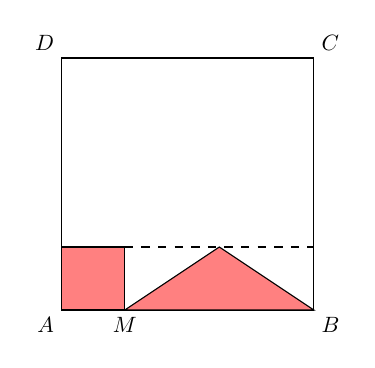
\begin{tikzpicture}[scale=\echelle,every node/.style={scale=\echelle}]
	\coordinate (A) at (0,0);
	\coordinate (B) at (4,0);
	\coordinate (C) at (4,4);
	\coordinate (D) at (0,4);
	\coordinate (M) at (1,0);
	\draw (A)--(B)--(C)--(D)--cycle;
	\draw[fill=\couleur] (A) rectangle (1,1);
	\draw[fill=\couleur] (M) -- (2.5,1) -- (B) -- cycle;
	\draw[dashed] (1,1) -- (4,1);
	\draw (M) node[below] {$M$};
	\draw (A) node[below left] {$A$};
	\draw (B) node[below right] {$B$};
	\draw (C) node[above right] {$C$};
	\draw (D) node[above left] {$D$};
\end{tikzpicture}
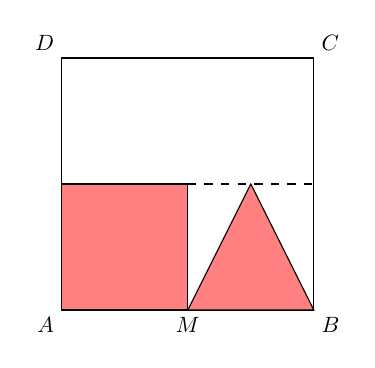
\begin{tikzpicture}[scale=\echelle,every node/.style={scale=\echelle}]
	\coordinate (A) at (0,0);
	\coordinate (B) at (4,0);
	\coordinate (C) at (4,4);
	\coordinate (D) at (0,4);
	\coordinate (M) at (2,0);
	\draw (A)--(B)--(C)--(D)--cycle;
	\draw[fill=\couleur] (A) rectangle (2,2);
	\draw[fill=\couleur] (M) -- (3,2) -- (B) -- cycle;
	\draw[dashed] (2,2) -- (4,2);
	\draw (M) node[below] {$M$};
	\draw (A) node[below left] {$A$};
	\draw (B) node[below right] {$B$};
	\draw (C) node[above right] {$C$};
	\draw (D) node[above left] {$D$};
\end{tikzpicture}
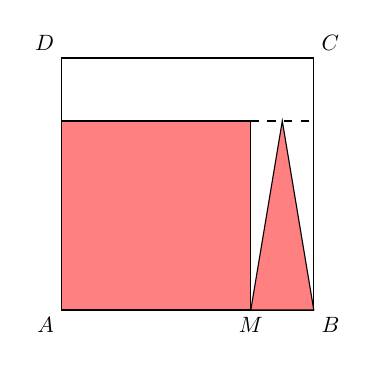
\begin{tikzpicture}[scale=\echelle,every node/.style={scale=\echelle}]
	\coordinate (A) at (0,0);
	\coordinate (B) at (4,0);
	\coordinate (C) at (4,4);
	\coordinate (D) at (0,4);
	\coordinate (M) at (3,0);
	\draw (A)--(B)--(C)--(D)--cycle;
	\draw[fill=\couleur] (A) rectangle (3,3);
	\draw[fill=\couleur] (M) -- (3.5,3) -- (B) -- cycle;
	\draw[dashed] (3,3) -- (4,3);
	\draw (M) node[below] {$M$};
	\draw (A) node[below left] {$A$};
	\draw (B) node[below right] {$B$};
	\draw (C) node[above right] {$C$};
	\draw (D) node[above left] {$D$};
\end{tikzpicture}

\exercice Dans quelle situation a-t-on l'aire du triangle la plus grande ?
\exercice Dans quelle situation l'aire du carré est égale à celle du triangle ?
\exercice Dans quelle situation l'aire du motif est elle égale à la moitié de celle de ABCD ?
\exercice Dans quelle situation a-t-on l'aire du triangle supérieure à la moitié de celle du carré ?
\exercice Comment évolue l'aire du motif en fonction de AM ? en fonction de MB ?
